\section{Literature review} \label{theory:literature-review}
In the search for related literature, we focused mainly on (L)DP mechanisms that can be used for general purposes (e.g. not only mean estimation), which is the most comparable to our mechanism.
The related literature is divided into three parts:
\begin{enumerate}
  \item Differential privacy and clustering: We explain how differential privacy is used for clustering.
  \item Differential privacy methods: We explore related literature for \gls{dp}.
  \item Cluster methods with (L)DP: We explore related literature for clustering with (L)DP.
\end{enumerate}
Afterward, we summarize the last two literature studies in a table.
This table includes components such as the type (LDP or DP) and whether a public code is available.

\subsection{Differential privacy and clustering} \label{theory:literature-review:dp-clustering}
There are different ways how to combine differential privacy with clustering \citep{baraheem_survey_2022}:
\begin{enumerate}
  \item Input perturbation: This method adds noise to the input data, so the clustering algorithms are trained on perturbed data.
  \item Output/label perturbation: This method adds noise to the output of the clustering algorithm.
        The model trains using the original data, and the noise is added to the output \citep{ji_differential_2014}.
        \item Gradient perturbation: The term gradient is used in machine learning algorithms that solve an optimization problem like deep learning \citep{hassan_differential_2019}.
        Perturbing the gradients ensures the optimization algorithm is private \citep{ji_differential_2014}.
  \item Objective perturbation: This method slightly differs from output/label perturbation but also adds noise to the output.
        The difference is it is added to the output of a loss function instead of the labels (for example, logistic regression) \citep{baraheem_survey_2022}.
\end{enumerate}
%This research aims to create a differential privacy framework training clustering on distributed data (See Section \ref{chapter:introduction}).
%The introduction explains that most differential privacy and clustering literature focuses on K-Means.
Many approaches targeting local differential privacy mechanisms must adapt the clustering algorithm (for example, k-Cluster) \citep{sun_distributed_2019}, which we explain later in this chapter.
For this reason, we concentrate on input perturbation in this study, as it allows a dataset to be used to train various clustering algorithms without modification.
\begin{figure}[H]
  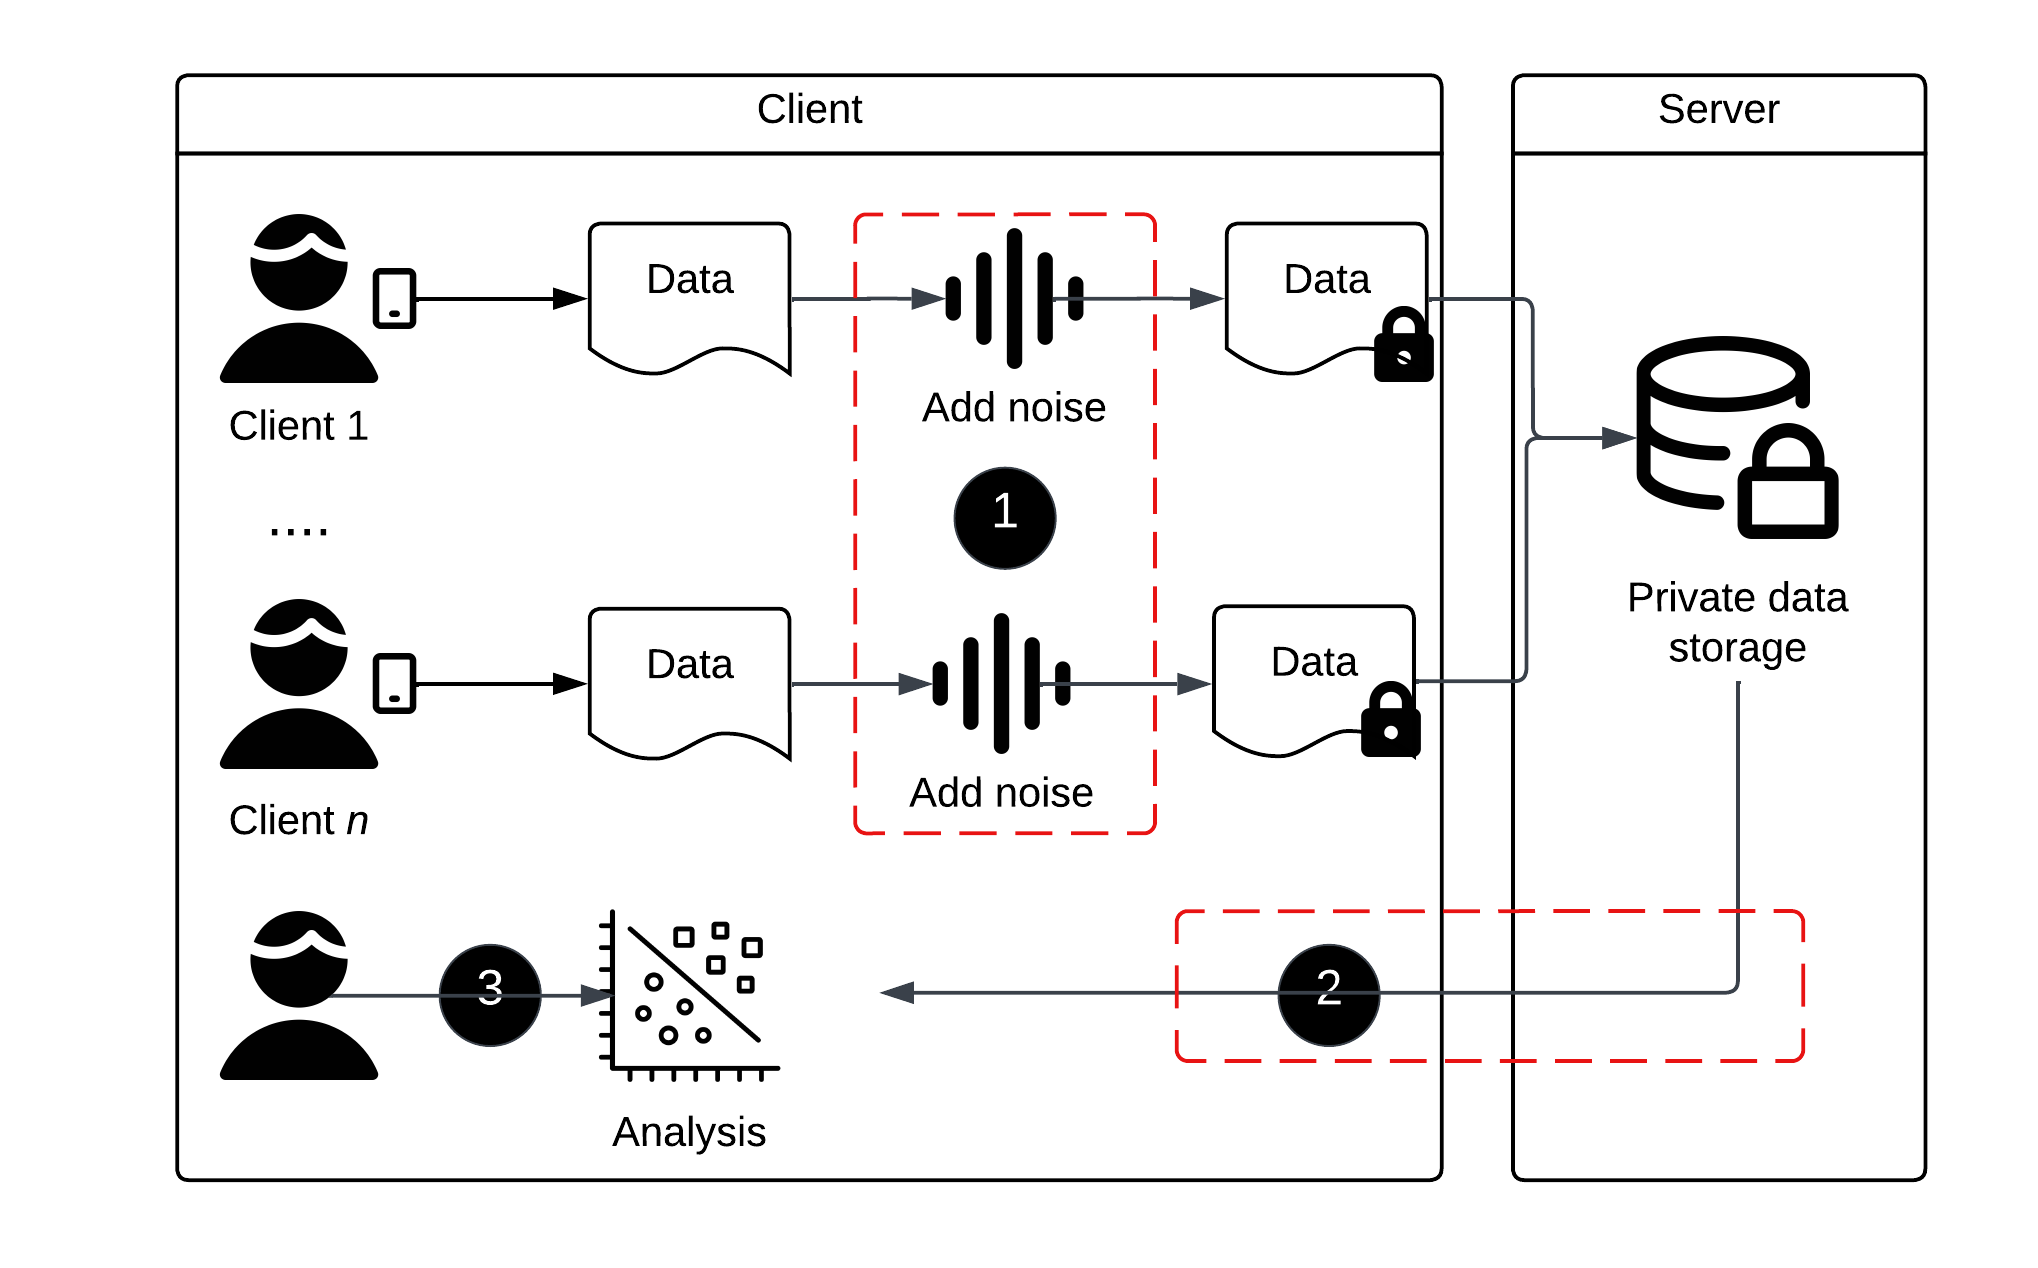
\includegraphics[width=0.75\linewidth]{TheorethicalFramework//ND-Laplace//Images/Thesis-nd - Page 7.png}
 \caption{Example on how our approach (1) of private training works for clustering and the \gls{ldp} setup from Section \ref{section:dp}}
  \label{fig:overview-clustering-and-dp}
\end{figure}
The above image shows where input/output perturbation would happen in the \gls{ldp} setup.
\begin{enumerate}
  \item Shows input perturbation. \textit{We use this approach for our research.}
  \item Shows where output perturbation happens, this would be part of the clustering process. Here the cluster labels perturbed, instead of the input.
Furthermore, we do not consider the perturbation variants 3 and 4, because they do not fit the research.

\end{enumerate}
The next section focuses on the differential privacy algorithms that are of interest to this type of input perturbation.

\newpage
\subsection{Differential privacy methods}
As discussed earlier, the Laplace method was the first to establish \gls{dp} \citep{dwork_differential_2006}.
The first paper we discuss is provided by Soria-Comas et al. and considers the distribution of the dataset for generating noise \citep{soria-comas_optimal_2013}.
Their work claims the Laplace mechanism is not optimal for a univariate function and aims at improving it by extending the Laplace mechanism.
The proposed method performs slightly better than Laplace on multivariate/multiple queries.

Quan et al. also proposed a new method to extend Dwork et al.'s Laplace algorithm \citep{geng_staircase_2015}.
They introduced the Staircase mechanism for 1-dimensional noise, which was later extended to support multidimensional data \citep{geng_staircase_2015}.
The mechanism aims to improve utility by adding the same level of privacy while adding less noise.
It represents a staircase-shaped \gls{pdf}, hence the name Staircase Mechanism (SM).
This mechanism accepts three configurable parameters comparable to those of the Laplace mechanism.
The authors' work can handle multidimensional numerical data and preserve the  $(\epsilon$)-differential privacy.
In the previous two paragraphs, we have mainly focused on the interesting literature regarding differential privacy.
Next, the succeeding paragraphs will mainly center on related literature concerning local differential privacy.\newline
%One disadvantage of the staircase mechanism is that it can produce an unbounded output, as noted by Wang et al. 
%This means that the perturbed data can exceed the original bounds of the data. 
%Additionally, the authors do not compare their results to comparable work in an experimental setting.

Nguyen et al. introduced a new \gls{ldp} mechanism for working with numerical data \citep{nguyen_collecting_2016}
Their primary focus is estimating means and frequencies on data and applying machine learning techniques such as Support Vector Machines (SVM) and linear regression using Empirical Risk Minimization.
Initially, the authors analyze Duchi et al.'s method \citep{duchi_privacy_2013} and highlight several shortcomings.
To address these issues, they introduce Harmony as a mechanism for \gls{ldp} perturbation.
This mechanism can perturb categorical and numerical data, providing high accuracy for classification and regression tasks.
To compare Harmony to other methods, they create the Hybrid Mechanism (HM), a combination of two existing methods for categorical and numerical data.
For this purpose, they extend other work \citep{bassily_local_2015} for perturbing multidimensional categorical attributes and use Duchi et al.'s method for numerical data \citep{duchi_privacy_2013}.
This combination of mechanisms allows them to compare their Harmony mechanism to the hybrid mechanism and measure the utility/accuracy differences.

Duchi et al. improved their method by formalizing the trade-off between statistical utility and (local) privacy, analyzing multiple estimation problems \citep{duchi_minimax_2017}.
Examples include mean, median, and density estimation.
To achieve this, they use minimax, a technique for finding the worst-case probability distribution.
Additionally, they focus on existing work and propose several optimization strategies.

Duchi et al.'s method was extended a couple of years later by adding support for bounded and multidimensional data \citep{wang_collecting_2019}.
The authors introduce the \gls{pm} to handle numeric and categorical data and the Hybrid Mechanism (HM), which combines \gls{pm} and Duchi et al.'s method for 1-dimensional data.
Their method's effectiveness is demonstrated using \gls{svm}, linear regression, and mean estimation.
\gls{pm} and HM are compared to Laplace and Duchi et al.'s solutions.
Optimized Unary Encoding (OUE) \citep{wang_locally_nodate} is also used for comparison, but for categorical data only, as the other methods do not support this.
% Instead of using the aforementioned techniques, categorical data is compared using frequency counting.

%\subsection{Geo-indistinguishability methods}
%\todo[inline]{Currently still work in progress}
\subsection{Cluster methods with (L)DP}
This chapter examines the various studies conducted on clustering in combination with differential privacy.
Initially, we looked at the most fundamental papers in this field. Subsequently, the focus shifted toward researching well-known papers published since 2020.

The first work we highlight was proposed by Nissim et al. and aimed at improving differential privacy methods, such as Laplace, which uses sensitivity to compensate the noise for a function \citep{nissim_smooth_2007}.
In addition to compensating the function, they also consider the dataset itself.
The algorithm is called "smooth sensitivity" and is used for instance-specific noise.
To apply it, the authors introduce a method/framework to calculate it effectively.
They use K-means, among other clustering algorithms, to demonstrate the method's effectiveness.
Their method requires the calculation of cluster distances using Wasserstein distance instead of Euclidean distance.
%Although, it preserves $(\epsilon, \delta)$-LDP it does not provide any experiments with real world datasets.

Another study focuses on interactive and non-interactive approaches for differential privacy in K-Means \citep{su_differentially_2015}.
The study builds upon the work done for DPLloyd, an interactive privacy extension of K-Means described by Blum et al. \citep{blum_practical_2005}.
The DPLLoyd mechanism partitions an n-dimensional dataset into a grid and releases the count for each grid by adding Laplacian noise to each count.
Another part of their research focuses on determining the width of the data cells.
The grid estimation method used in their research is called the extended uniform grid approach (EUG), and the complete K-Means method is called EUGkM.
The experiment evaluates it against the DPLloyd mechanism, which performs better in an interactive setting.
Therefore, they combine their algorithm for combining both aspects into a hybrid approach (EUGkM + DPLloyd approach) and show a better final performance.

The study of Nissim et al. researches finding the smallest possible radius in the Euclidean space  $R^d$ for a set of $n$ points \citep{nissim_clustering_2018}.
They propose a new solution that uses locality-sensitive hashing (LSH) for differential privacy to find 1-cluster in the $d$-dimensional Euclidean space.
This method works for differential privacy (LSH-GoodCenter), but they also extend this to the local model (LDP-GoodCenter).
The algorithm to find this radius is used to count the points enclosed by the radius, and Laplace noise is added to the count to preserve differential privacy.
The mechanism is combined and applied to work with the K-Means algorithm (LDP-K-Mean).
This mechanism was extended in a paper proposed by Kaplan et al. and introduced a similar LDP method \citep{kaplan_differentially_2018}.
They aim to reduce the number of interactions needed between the server and users to one, instead of the $O(k\log n)$ required for Nissam et al.’s solution \citep{nissim_clustering_2018}.
To increase the success probability, they use the same idea but extend it to have multiple centers instead of a single large one.
They call it the LSH-Procedure, and the algorithm Private-Centers is applied to generate centers to use with K-Means.
Then, they apply the same method to the LDP method initially proposed by Nissam et al. (LDP-GoodCenter).
The most recent work by Stemmer et al. focuses on improving the work done by Kaplan et al. \citep{kaplan_differentially_2018,stemmer_locally_2021}.
Because the original mechanism has a higher additive error, the noise added introduces a lot of error.
To solve this, the authors aim to reduce this error by improving the original GoodCenter algorithm \citep{nissim_clustering_2018}.
Their extended method is called WeightedCenters and also adds weights to candidate centers.
%So, in addition to calculating the centroids for each iteration, it also calculates the weights for each.
In the final iteration, the weights are used to create the K-Means or K-Median clusters.

Sun et al. proposed a mechanism for distributed clustering using local differential privacy (LDP) to preserve distance-based information.
They claim to have the first non-interactive LDP algorithm for clustering \citep{su_differentially_2015}.
This means they can perturb the data locally at once and send it to the server to cluster with both K-Means and \gls{dbscan} without interaction between data points.
They encode the client-side data into an anonymous hamming space using Bit Vector (BV) and modify the encoding to preserve Euclidean distance.
Their mechanism only shares distance information, so they could not use K-Means directly.
To overcome this, they modified the algorithm and called it K-Cluster.
Finally, the method is evaluated using Normalized Mutual Information (NMI) and Average Estimated Error (AEE).
%\todo[inline]{PrivBV}

Xia et al. noticed the shortcoming of Sun et al.'s work which is the need to share privacy-sensitive distance information \citep{xia_distributed_2020}.
Therefore, they create an interactive method for distributed K-means clustering using LDP.
The method converts features to binary strings and uses the Random Response mechanism (RR) to perturb each feature into a feature vector.
The privacy cost depends on the length of the bits of each feature transformation, meaning that a longer length yields more information at the expense of the privacy budget.
In each iteration, the serverside calculates and sends K-means centroids to each user, who recalculates distances until the centroids become stable.
The approach has the disadvantage of a high correlation between user data and the clusters.
To solve this problem, the algorithm is improved by having the client side send the user data and a set of random zero strings.
The server side then performs similar calculations to determine the actual cluster.
Huang et al. propose a private distributed K-means clustering algorithm for interval data that addresses a shortcoming in Xia et al.'s work by using Condensed Local Differential Privacy (CLDP) for small-scale values and LDP for large-scale values \citep{9679364}.
They preserve distance using a Square Wave (SW) mechanism and apply a classical K-Means algorithm on the server side to the perturbed data.
% TODO: Which shortcoming?

A recent mechanism that also builds around K-Means to preserve \gls{ldp} is called the LDPK mechanism \citep{yuan_privacypreserving_2021}.
As K-Means works only with numerical data, they use K-prototypes for supporting mixed data types.
The LDPK mechanism perturbs the user data first locally and interactively exchanges information with the server to complete the clustering process.
The mechanism they use for perturbation is the Harmony algorithm, proposed earlier by \citep{nguyen_collecting_2016}.
The S-Hist method is used to support categorical data, which was also introduced by Nguyen et al.
The server could still infer the correct information because of the correlation between the cluster centroids and the actual data.
Therefore, the author replaces S-Hist with OUE \citep{wang_locally_nodate} to improve accuracy.
To improve their mechanism further, the authors disturb the user’s cluster information with an extra extension to the LDPK method, called ELDPK.
For this purpose, they perturb the clusters with the GRR (Generalized Random Response) algorithm.
They show that the clustering quality increases if the data points increase. \newline

Most existing work focuses on (L)DP in combination with K-Means.
Finally, two interesting studies focus on differential privacy for \gls{ap} or \gls{dbscan}.
A study conducted by Cai et al. focuses on \gls{ap} \citep{cai_dp-ap_2020}.
Their method involves adding Laplace noise to the responsibility matrix.
For each sample data, a neighborhood is specified using a radius around the data point.
This area is called the neighborhood density, and each sample point’s preference value is adjusted according to its density value.
Higher density yields a higher chance of belonging to a cluster center and being ranked based on size.
The perturbed responsibility matrix and densities are combined and used to run AP.
They evaluated their method using the  \gls{ari}, Fowlkes-Mallows Index (FMI), and \gls{ami}.

Another study focuses on differential privacy for \gls{dbscan} \citep{bozdemir_privacy-preserving_nodate}.
The proposed solution involves clustering data between two or more parties using two servers.
Secure two-party computation (S2PC) is used to achieve this.
Using S2PC, both servers receive a random-looking secret share.
To recover the original data, both servers must combine their shares using S2PC, which combines the data without the servers having access to the full value.
The proposed protocol is privacy-preserving \gls{dbscan} (ppDBSCAN).
The calculations in this study are based on squared Euclidean distance (SED) and are evaluated using different methods.
To evaluate the performance of ppDBSCAN, the study compares its Adjusted Rand Index (ARI) to that of K-means.
%\subsection{Summary}
%\todo[inline]{Short summary}
\begin{landscape}
  \begin{table}[ht]
    \centering
    \begin{threeparttable}
      \begin{tabular}{rlllllllll}
        \toprule
        Paper                                      & Data type                  & Dataset                     & Code & Preserving               & Type    & Interactive     & Methods                    \\
        \midrule
        \citep{sun_privbv_2022}                    & -                          & Synthetic dataset           & -    & ($\epsilon, \delta$)-LDP & K-Means & Non interactive & -                          \\
        \citep{9679364}                            & -                          & -                           & -    & LDP                      & K-Means & Interactive     & -                          \\
        \citep{stemmer_locally_2021}               & numerical                  & -                           & -    & LDP                      & K-Means & Interactive     & -                          \\
        \citep{yuan_privacypreserving_2021}        & numerical                  & \makecell[l]{Adult dataset,                                                                                            \\ US Census dataset}                   & -                                                  & LDP                      & K-Prototypes        & Interactive     & LDPK and ELDPK                            \\
        \citep{bozdemir_privacy-preserving_nodate} & -                          & \makecell[l]{Deer dataset,                                                                                             \\ Lsun dataset, \\ S1}                  & -                                                  & DP                       & DBSCAN              & -               & ppDBSCAN                         \\
        \citep{cai_dp-ap_2020}                     & -                          & \makecell[l]{Iris dataset,                                                                                             \\ Seeds dataset}                        & -                                                  & DP                       & \gls{ap} & -               & DP-AP                            \\
        \citep{xia_distributed_2020}               & \makecell[l]{n-dimensional                                                                                                                          \\ numerical data}      & \makecell[l]{3D Road Network, \\ CarGPS}                           & -                                                  & LDP                      & K-Means             & Interactive     & LDPKmeans                        \\
        \citep{sun_distributed_2019}               & \makecell[l]{n-dimensional                                                                                                                          \\ numerical data}     & \makecell[l]{Aggregation dataset \\, Digit dataset, \\ Pathbased d...} & -                                                  & LDP                      & \makecell[l]{DBSCAN,\\  K-Means}     & Non interactive & \makecell[l]{Distance Aware \\ Bit Vector (DPBV)} \\
        \citep{nissim_clustering_2018}             & \makecell[l]{n-dimensional                                                                                                                          \\ numerical data}      & -                                                  & -                                                  & ($\epsilon, \delta$)-LDP & K-Means             & Interactive     & LDP-GOODCenter                   \\
        \citep{nissim_clustering_2018}             & -                          & -                           & -    & -                        & K-Means & Interactive     & \makecell[l]{LSH-Procedure \\ \& Private-Centers} \\
        \citep{su_differentially_2015}             & \makecell[l]{n-dimensional                                                                                                                          \\ numerical data} & \makecell[l]{Adult dataset, \\ Gowalla dataset, \\ Image dataset} & \tnote{a} & DP                       & K-Means             & Both            & \makecell[l]{EUGkM and hybrid \\ EUGkM + DPLloyd} \\
        %2011              & Differential privacy for location pattern mining                                                              & 2-dimensional geographical data      & Synthetic dataset with GPS trajectories            & -                                       & Differential privacy       & DBSCAN              & -               & DPQuadTree                                & -                                                                                                             \\
        \citep{nissim_smooth_2007}                 & \makecell[l]{n-dimensional                                                                                                                          \\ numerical data}             & -                                                  & -                                                  & ($\epsilon, \delta$)-LDP & K-Means             & Non interactive & Smooth sensitivity               \\
        \bottomrule
      \end{tabular}
      \begin{tablenotes}
        \item[a] \url{https://github.com/DongSuIBM/PrivKmeans}.
      \end{tablenotes}
    \end{threeparttable}

    \caption{Summary table of the literature review for (L)DP clustering algorithms.}
    \label{tab:summary_table_kmeans}
  \end{table}


  \begin{table}[ht]
    \centering
    \begin{threeparttable}
      \begin{tabular}{rllllllll}
        \toprule
        Paper                          & Data type                      & Dataset & Code      & Preserving    & Interactive     & Methods                  \\
        \midrule
        %2022                    & 3D Geo-Indistinguishability for Indoor Location... & 3-dimensional geographical data                    & -                                                  & -                                                  & Geo-indistinguishability   & Differential privacy method & -               & 3-dimensional Laplace mechanism & -                               \\
        %2019                    & Generalised Differential Privacy for Text Docum... & n-dimensional (?? data)                            & -                                                  & -                                                  & Differential privacy       & Differential privacy method & -               & n-dimensional Laplace mechanism & -                               \\
        \citep{wang_collecting_2019}   & \makecell[l]{n-dimensional                                                                                        \\ and 1-dimensional} & BR, MR  & \tnote{a} & LDP            & -                           & \makecell[l]{- Piecewise Mechanism (PM) \\- Hybrid Mechanism (HM)}                         \\
        \citep{duchi_minimax_2017}     & \makecell[l]{1-dimensional}    & -       & \tnote{a} & LDP           & -               & -                        \\
        \citep{nguyen_collecting_2016} & \makecell[l]{numerical, binary                                                                                    \\ and categorical data.} & BR      & -                                                  & $\epsilon$-LDP &                             & Harmony                                \\
        \citep{geng_staircase_2015}    & \makecell[l]{n-dimensional}    & -       & \tnote{b} & DP            & -               & Staircase mechanism (SM) \\
        \citep{geng_optimal_2013}      & n-dimensional                  & -       & -         & $\epsilon$-DP & Non interactive & -                        \\
        %2012                    & Geo-indistinguishability: Differential privacy ... & 2-dimensional geographical data                    & -                                                  & -                                                  & Geo-indistinguishability   & Differential privacy method & -               & 2-dimensional Laplace mechanism & -                               \\
        \bottomrule
      \end{tabular}
      \begin{tablenotes}
        \item[a] \url{https://github.com/forestneo/sunPytools/}.
        \item[b] \url{https://github.com/IBM/differential-privacy-lib}.
      \end{tablenotes}
    \end{threeparttable}

    \caption{Summary table of the literature review for (L)DP algorithms.}
    \label{tab:summary_table_dp}
  \end{table}

  \begin{table}
    \centering

    \begin{tabular}{rllllll}
      \toprule
      number & name            & samples    & features                      & target                & Source         & Realworld data? \\
      \midrule
      1      & Adult           & 48,842     & \makecell[l]{14 numerical                                                                \\ /categorical \\ /boolean}    & income (>50k, <= 50k) & UCI                                             & Yes             \\
      2      & Seeds           & 210        & 7 numerical                   & type                  & UCI            & Yes             \\
      3      & Iris            & 150        & 4 numerical                   & class (type of iris)  & UCI            & Yes             \\
      4      & CarGPS          & 17,785,500 & 3 geographical data           & -                     & -              & Yes             \\
      5      & 3D Road Network & 434,874    & 3 geographical data           & -                     & -              & Yes             \\
      6      & Pathbased       & 300        & 2 numerical                   & ground truth clusters & PapersWithCode & No              \\
      7      & Aggregation     & 788        & 2 numerical                   & -                     & -              & Unknown         \\
      8      & Digit           & 1797       & 8x8 numerical                 & number                & Scikit-learn   & Yes             \\
      9      & Lsun            & 400        & 2 numerical                   & ground truth clusters & -              & No              \\
      10     & S1              & 1500       & 2 numerical                   & ground truth clusters & -              & No              \\
      11     & Deer            & 20,033     & 2 numerical                   & -                     & -              & Yes             \\
      13     & Gowalla         & 6,442,890  & \makecell[l]{5 (geographical,                                                            \\ data, ids and time)} & -                     & \footnote{https://snap.stanford.edu/data/loc-gowalla.html} & Yes             \\
      \bottomrule
    \end{tabular}
    \caption{The different datasets used in the related literature.}
    \label{tab:datasets}
  \end{table}
\end{landscape}

